\ifdefined\included
\else
\setcounter{chapter}{3} %% Numéro du chapitre précédent ;)
\dominitoc
\faketableofcontents
\fi

\chapter{A Task planner making a robot compliant to human online decisions and preferences}
\chaptermark{A Task planner making a robot compliant to human online decisions and preferences}
\label{chap:4}
\minitoc


\section{Introduction}

\section{Related works}
paper Sonia UHTP



\section{Model of Execution}

    \subsection{Based on joint action literature}

    \subsection{Model description}

    \subsection{Model utility}

    \subsection{From Article}

\begin{figure}
    \centering
    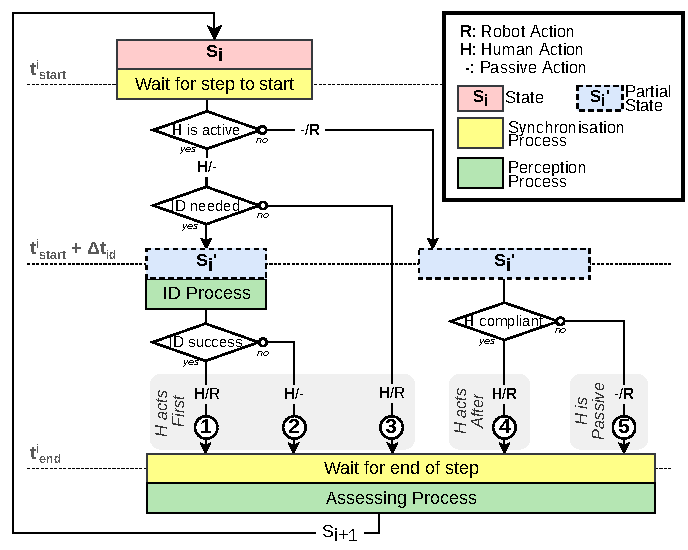
\includegraphics[width=\linewidth]{images/Chapter4/Execution_Automaton.drawio.pdf}
    \caption{
    The Model of Execution, in the form of an automaton and here simplified, captures the latitude of uncontrollable humans in their actions and guides our task planning approach.
    In this paradigm, the two agents can act concurrently but one is always compliant with the other's decision to act.
    Here, the human is always free to decide whether to start acting first, or after the robot, or not to act at all.
    To be compliant, the robot attempts to identify human decisions using perception and situation assessment as well as possible collaborative human signaling acts (e.g., gestures or speech).
    }
    \label{fig:model_of_execution}
\end{figure}

Our task planning approach uses a model of execution to improve the fluency and amenability of HRC. 
This model is in the form of an execution controller as shown in Figure~\ref{fig:model_of_execution}, and is based on several key notions and mechanisms borrowed from studies on joint actions~\cite{Sebanz-2016,kourtis2014attention}, and adapted to Human-Robot Joint Action~\cite{clodic-2017,curioni-2019}.
The key idea is that co-acting agents co-represent the shared task context and integrate task components of their co-actors into their own task representation~\cite{Schmitz-2017, Yamaguchi-19}. Also, coordination and role distribution rely strongly on reciprocal information flow, e.g., social signals~\cite{curioni-2019}, prediction of other's next action~\cite{luke-2018}.

Our proposed execution model is implemented on a robot that co-acts with a human, integrating explicit representation and exploration of the task representations for the robot and for the human. 
It also identifies precisely how reciprocal information flow is used in task execution (detecting and interpreting human actions, signals produced by the robot while acting, and also when the robot waits for human actions or their signals).

Another essential question is the criteria for choosing the next action, or more globally, how to share the load between the two co-actors. The choice depends on the context and actors' preferences~\cite{Gombolay-2015, Strachan-2020,Curioni-2022}. 
Concerning the case when one actor is a robot, we think it is important to provide a standard default behavior of the robot where the robot does its best to reduce human load but still leaves full latitude to act whenever humans want. 
Our scheme provides this ability and also allows humans to inform about their preferences at any moment.

Consider an example to clarify the execution automaton. 
Assume a human and a robot have to pick up two blocks, \textit{A} and \textit{B}, that both can reach. 
They can pick it up both at the same time unless they try to pick up the same block, which causes conflicts between their actions. 
As a result, despite being executable in parallel, the actions are interdependent, and in order to avoid conflicts, one agent must be compliant with the other. 
However, if we consider a third block \textit{C} that only the robot can reach, it can always pick up this block without any risk of conflicts with the human's choice. 

In a state, a human decision can result in one of three outcomes.
First, the human can choose to act first (\textit{left~subtree}).
If the robot's best action is not in conflict with the human action (e.g., \textit{pick~C}), the robot can safely perform this action concurrently with the human operator (\textit{branch~3}).
However, if the robot's best action is either \textit{pick~A} or \textit{pick~B}, the human action must be identified first with a subroutine in order to be compliant with it.
If this subroutine is successful the robot can perform any action which is congruent with the identified human action (\textit{branch~1}). 
This includes the robot's choice to be \textit{passive} and let the human act alone. 
However, if the robot is unable to identify the human action, it must remain passive in order to avoid potential conflicts (\textit{branch~2}). 
Then, the human can either decide to be \textit{passive} or to act after the robot (\textit{right~subtree}). 
In both cases, the human is \textit{passive} at the beginning, making the robot to start performing alone a feasible action. 
While the robot is acting, the human is free to remain \textit{passive} until the next step (\textit{branch~5}), or to choose a congruent action to act concurrently (\textit{branch~4}). 
As a result, the human can always choose to 1) act first, 2) act after the robot, or 3) not act at all. 
The robot will always be compliant with these online human decisions.

When both agents finish their actions, the step is considered as \textit{``over''}. 
Then, another subroutine assesses the new world state ($s_{i+1}$), which is the result of the concurrent actions being executed in the state $s_i$, before repeating the whole process until the task is solved.

Note that if both agents are passive (the human decides to be passive when the robot cannot act) then the step is repeated. 

\section{Problem specification + solution}

    \subsection{Problem}

Belief divergences are out of the scope of this particular work. Hence, for simplicity reasons, we consider the two beliefs (robot and estimated human ones) as always aligned, and they are represented as a unique world state. However, we are convinced that this work could be adapted easily to consider the two distinct beliefs.

The problem is specified as follows. One initial world state, described using state variables. Distinct human and robot action models described with HTNs. Distinct human and robot initial agendas. 

[More details about each]

    \subsection{Solution}

A Planning state, referred as p-state, corresponds to a state in which the planning problem is while progressing toward a solution. A p-state contains the current world state (aligned beliefs of the agents) and the respective agenda of the human and the robot. Thus, keep in mind that p-states are very different from world states.
The initial p-state is formed using the initial human-robot agendas and the initial world state given in the problem specification. P-states are connected with each other through concurrent pairs of human-robot actions. Note that we consider passive actions, hence, there may be only one active agent in a pair if concurrent human-robot actions. A goal p-state is characterized by a world state satisfying given goal conditions and by empty agendas.
The exploration produces a directed acyclic graph, referred as the search graph, from the initial p-state to several goal p-states through sequences of concurrent action pairs. Thus, any path from the root to a leaf is a possible plan. Once the exploration done, search graph computed, another process extract the optimal robot policy from the graph. In the manner of an AND-OR tree, this policy indicates for all p-states the best concurrent robot action (OR node) to execute to be compliant with any possible human action (AND node).

Clarification of the directed acyclic graph. Nodes represent p-states and are connected with each other through directed edges representing human-robot concurrent action pairs. However, for practical reasons action pairs are considered as nodes of the graph having only one parent p-state node and one child p-state node. Consider that each directed edge between two p-state have one unique intermediate action pair node. The graph has one root node (no parent) which is the initial p-state. All leaf nodes (no children) represent a goal p-state. 

It is one of our design choice to do not consider explicit action costs and perform an exhaustive offline search to produce this search graph in order to solve a problem. Since the policy generation is very quick it allows generating and updating the robot policy online according to human feedbacks. 




\section{Exploration}

This section details how the exploration happens, and thus, how the search graph is generated. This requires several sub-process which are each detailed here. First, the overall exploration process is presented, and next subsections provide details on the sub-processes mentioned in the overall process.

    \subsection{Overall process}

We keep track of the p-state to explore, this set being initialized with the initial p-state. Then, until the set is empty we select one and explore it.
First, from this selected p-state, every possible concurrent human-robot action pairs are computed considering both agendas, the world state and reasoning on the compatibility of the actions in terms of preconditions and effects. This process requires several sub-steps and is detailed later. Thus, we obtain several action pairs leading to the same amount of new p-states (with updated world state and agendas).
Second, we check if any of the newly created p-state are similar to any existing p-state. If so, we can "merge" them to avoid redundant computations. To do so, we basically keep track of the unique p-state already checked and for each new p-state we check if it is similar to one of the already checked one. 
If not, the new p-state is added to the set of already checked p-states. 
If a similar one is found, the new p-state is deleted and the action pair leading to it is connected to the existing p-state instead.
Eventually, the remaining new p-states are added to the set of p-states to explore. 
When the set of p-states to explore is empty then the exploration is over and the graph obtained corresponds to the "search graph" where any path from the initial p-state to a leaf corresponds to a possible execution trace / plan.

    \subsection{Compute next agent actions}

From a p-state, more precisely from a world state and an agenda, we can estimate what are the next action an agent is likely to perform. Doing so is referred as the refinement process. To do so we use the corresponding action model in the form of an HTN. Here the agendas are considered as list of abstract or primitive task, where primitive task can be executed (actions), and abstract ones can be decomposed into several others subtasks. 
The refinement process consists in applying applicable methods of the first task of the agenda until it is primitive. When several methods are applicable they are all applied in a distinct refinement trace.
Eventually, for each different sequence of applied method we obtain a new agenda starting with a primitive task. For each such primitive task we create a copy of the world state contained in the given p-state, and we applied the correspond action, updating the world state. 
Hence, for each possible action a new p-state is created with the refined agent agenda, the unchanged other's agenda and the updated world state. 
Note that this process can "generate" default passive actions in several cases. First, when an agent's agenda is empty an \textit{IDLE} passive action is inserted as the first primitive task in the agenda. This means that the agent has nothing to do and thus is likely to remain passive. Either when there are no applicable methods or when the primitive task is not applicable then a \textit{WAIT} passive action is inserted. This means that the agent has still something to do but cannot do it currently. Note that when computing the concurrent pairs of action we also add the \textit{PASS} action which corresponds to the agent being voluntary passive, despite having something to do. Note also that these different passive action types just help to better understand the generated plans, but they are treated equally / similarly in the planning process.

    \subsection{Concurrent action pairs computation}

This sub-process is computes from a given p-state all possible concurrent action pairs that may be executed. It is based on the previously described refinement process. This main objective of this sub-process is to identify the next actions the agents are likely to perform to reach the goal and identify which of them can be executed in parallel. The classical way to do such reasoning is by analyzing the preconditions and effects of the two actions and determine if there are conflicts between them, e.g., the effects of the first action makes the preconditions of the other false.
However, our current python implementation of the planner is convenient but has no "explicit" preconditions and effects. Everything is defined through python function. The effects of an action are a function with a world state as input and returns the updated world state. Action preconditions are functions with a world state as input and return a boolean. And methods (of an associated abstract task) are functions with world state as input and return a list of tasks to update the agenda with. Methods also have preconditions working similarly then action preconditions. 
Hence, it's challenging to extract the explicit effects and preconditions of an action. That is why we decided to rely on an assumption to check the compatibility of concurrent actions. 
We consider the following in a given state. 
If action 1 and action 2 can be sequentially performed in both orders (1$\rightarrow$2 and 2$\rightarrow$1). Then we can assume that there are no causal links between the two actions and that they can be performed concurrently. The only care to take are shared resources such as a tool that would only be used during the action, making it available before and after but not during the action. To tackle this issue, shared resources are explicitly declared in the world state and in the action models. Two actions requiring a same shared resource cannot be parallelized.
One benefit the way we check if two actions are mutually exclusive is making the actions estimations a black box. Indeed, we can easily replace the way we estimate the next actions each agent is likely to perform. Especially for the human, we could use a pretrained human activity estimator neural network, or more classical planner like PDDL. 

With the causal principle above in mind, we proceed as follows to compute the possible concurrent action pairs from a given p-state. We start by estimating all possible human actions by refining the human agenda, generating a new p-state for each possible action. For each such p-state we first create an action pair where the robot is passive by inserting a \textit{PASS} robot action. This \textit{PASS} pair is stored among all other "human pass pairs". Second, we refine the robot agenda to obtain all feasible sequences of human then robot actions and their associated p-states. We refer to them as the sequential human starting pairs. In a symmetrical way we compute the sequential robot starting pairs and "robot pass pairs" by starting with the robot then refining the human agenda.

Eventually, every action pair which is present in both the human and robot starting pairs are extracted and added to a set of concurrent action pairs. 
Additionally, here passive action are always parallelizable. Indeed, the only case where this couldn't be the case is when considering "joint actions" requiring the two agents such as lifting a table/object together. For now, such actions are not considered. Thus, the two sets of \textit{PASS} pairs are directly added to the set of concurrent action pairs. 
Lastly, a double passive pair with two PASS is generated and added to the concurrent set. This pair is special since it doesn't update the world nor the agendas, hence, it leads back to the previous p-state without progressing toward the goal. These pairs not need to be explored and help it different ways. First, it helps the execution for instance when only the human can act but decides anyway to pass voluntary. Then the policy will natively stay in the same p-state. Second, it is easy to detect dead-ends which correspond double \textit{WAIT} pairs. In such case, both agent cannot act, due to the lack preconditions for action or decomposing an abstract task, and they remain stuck without solving the task.  
Last, double \textit{IDLE} pairs indicates that both agendas are empty and thus that the task should have been solved. 

The obtained set of concurrent action pairs corresponds to all possible concurrent action that the human and the robot can execute in parallel in the initially given p-state. Each possible pair leads to a new p-state with updated agendas and world state, creating a tree structure. 

    \subsection{Merging p-states}

Although the tree structure produced by the process described above is complete and sound, it is inefficient and scales badly. Indeed, during the exploration we are likely to encounter several times similar p-states. For instance, consider an action pair where both the human and robot are active leading to a new p-state, one branch. Now, consider a first action pair where only the human is active, and a second where only the robot is active. Performing those two last pairs in both orders creates two other branches. However, even though the trace is different, the three p-states are identical (same world state and agendas) and it's highly redundant to explore independently each of them. That is why after each computation of the concurrent action pairs we check if any of the newly generated p-state is similar to an existing one, and if so, we connect the corresponding pair to the existing p-state to avoid redundant explorations. Doing so we transform the tree structure into a directed acyclic graph (on the condition that we don't consider double \textit{PASS} cycles). In the manner of a tree, we will refer to nodes without child as leaves nodes, which are goal p-states. Hence, now, each leaf can be reached with several paths. 
When looking for similar existing p-state, we assume that p-states which are parent with the new p-state, directly of not, will necessarily be different, and thus they are excluded. This speeds up the comparison process. 



\section{Policy generation}

First of all, as depicted in figure~\ref{fig:and_or}, all children concurrent action pairs of a p-state can actually be seen as an AND-OR graph. Since we want to preserve the latitude of choice the human have at execution, each possible human choice of action is considered as an AND edge and leads to a partial p-state. And from a partial p-state, each compliant concurrent robot action is considered as an OR edge and leads to another p-state.

Thus, generating the robot policy $\Pi$ consists in identifying the best concurrent compliant robot action $RA^*$ for each possible human action, or partial p-state $ps_i^j$.

These best concurrent robot actions are determined by aiming to optimally satisfy an estimation of the human preferences regarding the task. Eventually, at execution, the human is free to perform any of the explored action and the robot will accordingly perform an optimal concurrent action to both solve the task and satisfy their estimated preferences.

Hence, before giving more details about the policy itself, we first describe the format of human preferences, how we could estimate them, and what it allows us to do. After, we describe the actual process to generate the robot policy from the search graph using the estimated human preferences


**The robot policy consist in performing the best robot action according to the node and the human action, i.e., robot action stored in the "best compliant" pair corresponding to the human action.
If all "best compliant" pair have the same robot action, the robot can perform as soon as the step stars, otherwise the human action must be identified.**

\begin{figure}
    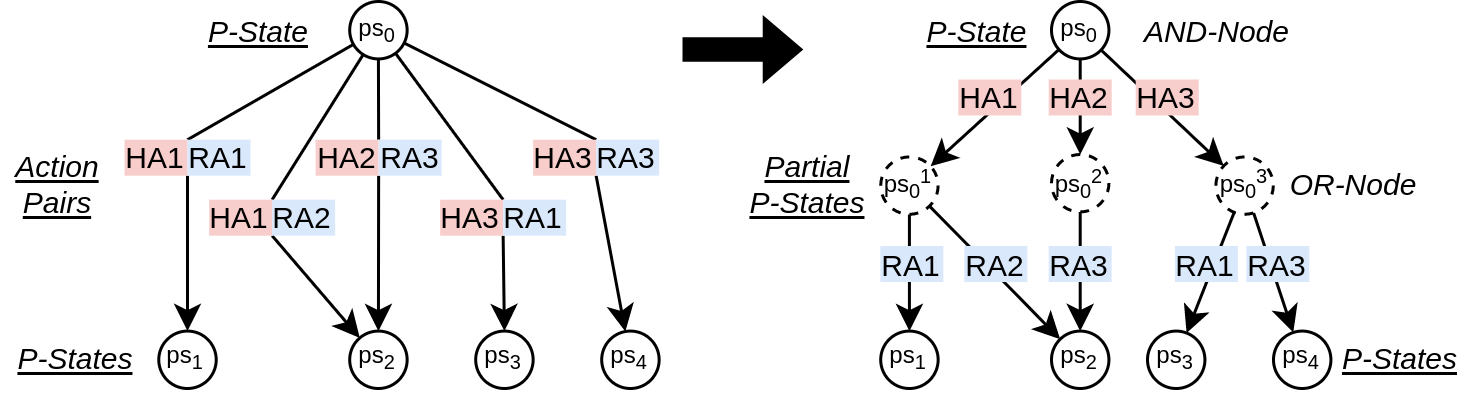
\includegraphics[width=\linewidth]{Chapter4/and_or_tree.png}
    \caption{AND-OR graph representation of the action pairs. 
    The robot policy must be compliant to any decision of the human. Hence, the problem can be seen as an AND-OR graph where for each possible human choice of action (AND node), we must determine the best concurrent robot action among the possible robot actions (OR node).
    }
    \label{fig:and_or}
\end{figure}


    \subsection{Estimated Human preferences}
estimations, format, Discussion(often inaccurate, hence our Approach), consider metrics, is a prioritized sequence of metrics to max or min, allow comparison of metrics

In this approach, instead of trying to minimize action and social costs, which are challenging to estimate accurately and quantitatively, we decided to aim at satisfying an estimation of the human preferences. In a way, the costs are included / covered / reflected in the human preferences. Our approach is to characterize each possible trace with a set of various metrics such as follows:

\begin{itemize}
    \item \textbf{Time of Task Completion}: Time step at which the task if achieved.
    \item \textbf{Time of End of Human Duty}: Time step after which the human can remain passive.
    \item \textbf{Human Effort}: Number of non-passive human action.
    \item \textbf{Global Effort}: Number of non-passive human and robot action.
    \item \textbf{*Passive While Holding}: Number of steps where an agent is passive while holding a cube.
    \item \textbf{*Number of Drop}: Number of times an agent drops cube (place back a cube on the table, not in the stack).
\end{itemize}

Note that general metrics are complemented with additional domain specific metrics (marked with a star *), given in the problem specification. The set of metrics helps to characterize and evaluate each possible plan / trace. However, even if the possible plans are characterized we so far have no way to compare them and find the best one. Doing so requires additional criteria indicating how to prioritize and compare the different metrics.

That's where we consider an estimation of the human preferences to allow us to the plans and which are given by any mean external to our system. The preferences can be estimated or also given, verbally or not. Here, we consider the human preferences in the following form. These preferences are an ordered list of the metrics characterizing the traces. Note that it's not necessary for all metrics in the list above to be present, but only them can appear in the preferences. This ordered list indicates if each metric should be maximized or minimized, and in which order / with which priority. For instance, assuming the preferences aim to minimize all metrics, the best of two given plans is the one with the lowest first metric of the list. If the two plans have equal first metric then we use the second metric, and so on. Here are two arbitrary examples of human preferences trying respectively to finish the task as fast as possible and to minimize the human effort (all metrics are minimized):

TTC - GE - HE - TEH - PWH - ND 

HE - TEH - TTC - GE - PWH - ND 

Note that estimating either human preferences or explicit action and social costs is challenging and is hardly accurate, those are very context dependent and can even vary over time.
Being aware of this, we use the estimated human preferences as a guide for the robot behavior, but we also make sure to be compliant to the human activity to lessen in impact of a wrong estimation. 

    \subsection{Process}

\begin{figure}
    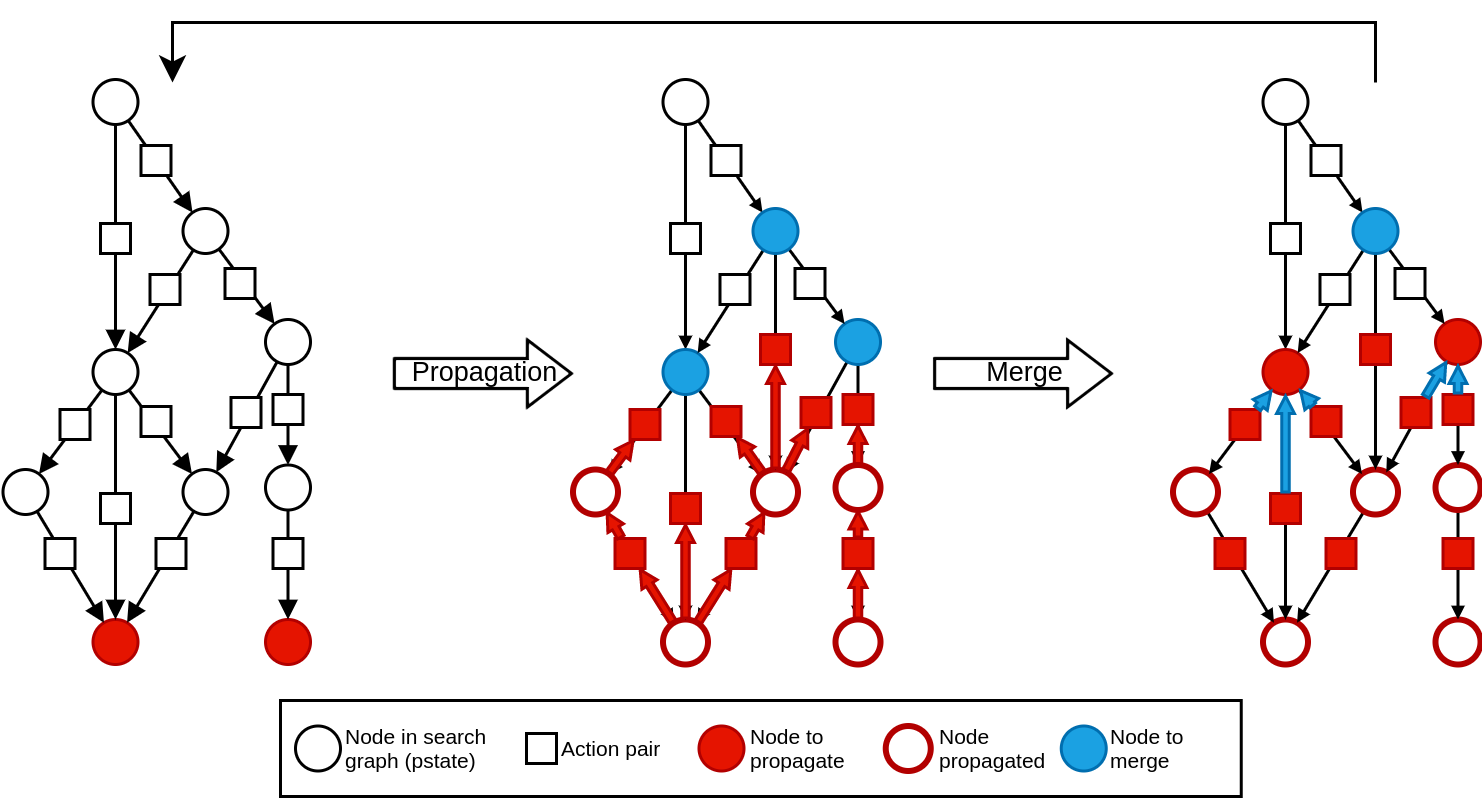
\includegraphics[width=\linewidth]{images/Chapter4/policy_generation.png}
    \caption{Policy generation process illustration on an arbitrary search graph. Propagation and Merge processes repeat until all nodes are marked as propagated.}
    \label{fig:policy_generation}
\end{figure}

To generate the robot policy from the search graph we proceed from the leaves to the root. We compute the set of metrics for each possible trace, and when reaching nodes with several children we compare the metrics of the different traces, identify the best ones to update the robot policy with, and then we continue by propagating only the best set of metrics.
This process is achieved by repeating two sub-routines detailed just below, namely: Propagation and Selection. 

\begin{algorithm}
\caption{Policy Generation}\label{alg:policy_generation}
\begin{algorithmic}[1]

\State \textbf{input}: $leafNodes$ \Comment{Set of all leaf nodes from the search graph}
\State $nodesToPropagate \gets \emptyset$
\State $nodesForSelection \gets \emptyset$

\State $Initialization(nodesToPropagate, leafNodes)$

\While{ $nodesToPropagate \neq \emptyset$ and $nodesForSelection \neq \emptyset$ }
    \State $Propagation(nodesToPropagate, nodesForSelection)$
    \State $Selection(nodesToPropagate, nodesForSelection)$
\EndWhile

\end{algorithmic}
\end{algorithm}

    \subsubsection{Format and Initialization}

During this process we compute and store the best reachable set of metrics alternatively in the p-states and in the action pairs. Initially, we store default/null metrics in every leaf p-state. Then we keep track of two types of nodes. First, keep track of the nodes which metrics should be propagated in the next step, those are stored in the set $\{nodesToPropagate\}$ which is initialized with all leaf nodes. This set is populated by the Selection sub-routine. Secondly, we keep track of the nodes to that should select among several the best set of metrics, and thus, the best actions to perform, this set is $\{nodesForSelection\}$. This set is populated by the propagation sub-routine and is being emptied by the selection sub-routine. The process is over when the two sets are empty, thus, when they are no more nodes either to propagate nor for selection.

    \subsubsection{Propagation}

This sub-routine consists in picking a node to propagate from the set $\{nodesToPropagate\}$. For each parent action pair of that node we create a copy of the set of metrics of the propagated node and update them according the parent action pair and propagated node. 
The metrics must be cumulative. 

Examples for rules to update the metrics are the following. If the human action of the pair is not passive then the \textit{Global Effort} and \textit{Human Effort} metrics are both incremented by 1. If the pair isn't a passive \textit{IDLE}-\textit{IDLE} then \textit{Time of Task Completion} is incremented by 1. If the robot action is passive in the pair and if in the child p-state the robot is holding a cube then \textit{Passive While Holding} is incremented by 1. 

Rules to update the standard metrics are the following \textbf{TO UPDATE, THERE IS AN OFFSET OF 1 FOR TIME STEP METRICS}:
\vspace{-\topsep}
\begin{itemize}
    \setlength\itemsep{-0.3em}
    \item Always increment (by 1) \textit{Time of Task Completion}%
    \item If the human action is passive and the current \textit{Human Effort} is zero, then the temporary metric \textit{Number Last Passive Human Action} is incremented.
    \item \textit{Time of End of Human Duty} = \textit{Time of Task Completion} - \textit{Number Last Passive Human Action}.
    \item If human action is not passive, then \textit{Human Effort} and \textit{Global Effort} are incremented.
    \item If robot is not passive, then \textit{Global Effort} is incremented.
\end{itemize}
Rules to updates domain specific metrics, must be provided:
\vspace{-\topsep}
\begin{itemize}
    \setlength\itemsep{-0.3em}
    \item If human action is passive and in child p-state the human is holding a cube, then \textit{Passive While Holding} is incremented.
    \item \textit{(Similarly with the robot)}
    \item If the human action is to drop a cube back on the table, then \textit{Number of Drop} is incremented.
    \item \textit{(Similarly with the robot)}
\end{itemize}

The updated metrics are stored in their corresponding action pair. Then, two cases can occur for each parent action pair with stored metrics, referred as propagated pairs. First, if the parent node of the propagated pair has more than one child then we add this parent node to the set $\{nodesForSelection\}$. Otherwise, the metrics of the action pair are stored in the parent node which is also added in the set $\{nodesToPropagate\}$. 
% In both cases, the former propagated node is marked as ``propagated'' (not needed actually).
The sub-routine repeats until the set $\{nodesToPropagate\}$ is empty.

\begin{algorithm}
\caption{Propagation}\label{alg:propagation}
\begin{algorithmic}[1]

\While{ $nodesToPropagate \neq \emptyset$ }
    \State $N \in nodesToPropagate$
    \State $nodesToPropagate \gets nodesToPropagate \setminus \{N\}$
    \For{ each $P$ in $N.parents$ }
        \State $P.metrics \gets CopyAndUpdateMetrics(N.metrics, N, P)$
        \If{ $HasOneChild(P.parent)$ }
            \State $P.parent.metrics \gets P.metrics$
            \State $nodesToPropagate \gets nodesToPropagate \cup \{P.parent\}$
        \Else
            \State $nodesForSelection \gets nodesForSelection \cup \{P.parent\}$
        \EndIf
    \EndFor
\EndWhile

\end{algorithmic}
\end{algorithm}



    \subsubsection{Selection}

Introduce policy notation, p-state and partial p-state (AND-OR tree)

When a node has several children, possible action pairs, then we must evaluate and compare them in order to make the best robot choices and update the policy with them. The evaluation is part is done by the propagation sub-routine. The Selection one checks when robot choices are ready to be made, update the robot policy and prepare the next propagation phase. 

More precisely, this sub-routine checks every node in the $\{nodesForSelection\}$ set to know if we are ready to make a choice, i.e., if every child pair of that node has metrics stored in it, has been propagated. 
If not, nothing happens and the node remains in the set.
If so, we are ready to compare the pairs and update the policy. Since we want the human to be free to perform any action, even suboptimal, we must find the best concurrent robot action for each possible human action. The first step is to group/sort/organize the children pairs by similar human action. Then, for each group of pairs, we compare their metrics using the estimated human preferences and identify the best pair of the group, which is marked a ``best compliant pair''. After, all marked pairs are compared the overall best pair is identified and marked as ``best pair''. Eventually, the metrics of the ``best pair'' are stored in the node from $\{nodesForSelection\}$, the node is removed from the set and added to the other set $\{nodesToPropagate\}$.

\begin{algorithm}
\caption{Selection \textbf{To update with policy notations}}\label{alg:selection}
\begin{algorithmic}[1]

\For{ each $N$ in $nodesForSelection$ }
    \If{ $ReadyForSelection(N)$ }
        \State $groups \gets GroupPairsByHumanAction(N.children)$
        \For{ each $group$ in $groups$ }
            \State $P = IdentifyBestPair(group)$
            \State $MarkAsBestCompliant(P)$
        \EndFor
        \State 
        \State $bestCompliantPairs \gets RetrieveMarkedBestCompliant(N)$
        \State $bestPair \gets IdentifyBestPair(bestCompliantPairs)$
        \State $MarkAsBest(bestPair)$
        \State 
        \State $N.metrics \gets bestPair.metrics$
        \State $nodesForSelection \gets nodesForSelection \setminus \{N\}$
        \State $nodesToPropagate \gets nodesToPropagate \cup \{N\}$
    \EndIf
\EndFor

\end{algorithmic}
\end{algorithm}

\section{Results}
simulation of execution, without durative action

    \subsection{concept of aligned-adversarial pairs of prefs/estimations}

    \subsection{results}

\section{Discussion and Limitations}
\section{Conclusion}




